\chapter{State of the Art}

% AMAIA: For the state of the art, I think that you should re-organize it to cover the main different challenges of video analysis, and explain what people do to tackle each (even though you end up citing the same paper more than once in the process). You should also explain what you do in your project, and how it resembles or differs from what others did.

% 1. How do people use information in different frames? Some use 2D convolutions and merge them somehow, others use 3D conv. Here you can talk about pretrained networks (some people use VGG imagenet, there's people who have trained other models for Sports1M, right?)
% 2. How is motion encoded ? Some works directly use optical flow, while others directly input the visual data.
% 3. How do people ensure temporal consistency? LSTMs or GRUs
% 4. Particularly for activity detection, how do people do this? I remember the paper from columbia, where there are several stages. Maybe a strength of your work is that you train a single network that does it all (you just postprocess the output).
% ...


Many works in the literature have explored activity and action recognition problems using deep learning strategies. Most of them can be classified by the deep learning techniques used. Most of them used an approach of two stages (encoder and decoder) to learn from video's dataset. The first stage, the one being consider a decoder, is the stage that tries to encode the visual and temporal information from the input videos into some features vectors or information. The second stage, also known as decoder, tries from the extracted encoded information from the first stage, make a prediction of the output, which can be a classification of the video or a temporal localization of an activity.

Is very common see that as encoder, use Convolutional Neural Networks (or also known as CNNs) as it has been widely demonstrated that applying CNN networks to images and videos has obtain very good results in classifications tasks. A very well known and used CNN network is the VGG\cite{Simonyan14c} network which was top scored on ImageNet Challenge in 2014 on classification task. This network uses 2D convolutional kernels to extract spatial correlations from images and therefor learn how to classify them. 

Applying this techniques to activity detection, there are some implementations of using 2D Convolutional Neural Networks over the frames\cite{gkioxari2015contextual}\cite{yeung2015end}\cite{ballas2015delving} to extract spatial correlations into the video data. As the video also present temporal correlation, different approaches have been tried to exploit it. The first approach you can find on the literature is to weight the frames at the input\cite{yeung2015every} so information of a chunk of frames is given to the neural network. 

\begin{figure}[ht]
\begin{center}
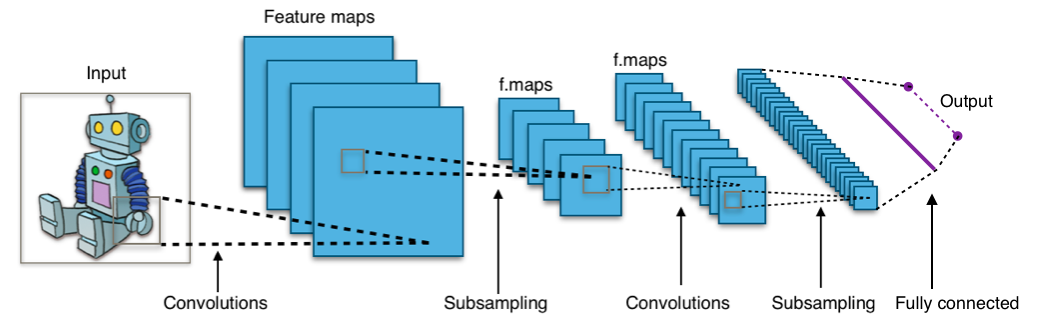
\includegraphics[width=1\linewidth]{img/stateofart/cnn_architecture}
\end{center}
\caption{Example of the Architecture of a Convolutional Neural Network}
\label{fig:cnn_architecture}
\end{figure}

In addition to this technique, it can be found the computation of the optical flow a solution to codify temporal correlations to train convolutional neural networks\cite{simonyan2014two}\cite{Ng_2015_CVPR}. This techniques extract temporal information but they are limited to the amount of information a 2D space can give, and without letting learn the neural network about temporal information. 


% AMAIA: I think it's a good idea to cover the cited works in more detail. What are their differences? What do they have in common? Do you take ideas from them? What are the differences between what they do and what you do?

On the other hand very recently was proposed a CNN which tries to exploit both spatial and temporal correlations using exclusively a Convolutional Network and having all the frames as input. This is the 3D convolutional network, also referenced as C3D\cite{tran2014learning}. This network uses 3D kernels rather than 2D to extract videos information and try to learn from the 3 dimensions. It has been widely used\cite{baccouche2011sequential}\cite{tran2015deep}\cite{tran2014learning}\cite{shoutemporal} for applications such as video classification. On some other research papers\cite{yao2015describing}\cite{zhang2016modelling} the both approaches have been tried using 2D and 3D convolutional networks.

For this C3D network, the input data are clips of videos which all the frames are provided without any previous codification and even it has been proposed a combination of 2D and 3D Convolutional Neural Networks\cite{Ng_2015_CVPR}\cite{yao2015describing}. Also it has been tried to extract motion 3D features from videos to then give as input of the 3D CNN\cite{yao2015describing}. 



% REMOVED: For this network, the input data is very common to use the raw video and let the network learn and extract information. Feeding the network with all the pixels of each frame in bunches of frames (the C3D is fed up with a 16 frame video clip) is very common, but in other cases some tricks are done. To feed up 2D convolutional layers but trying to learn from temporal correlations, what is done is compute the optical vector between frames and give it to a 2D CNN for training in combination with a parallel CNN fed up with the raw frames\cite{Ng_2015_CVPR}\cite{yao2015describing}.

In addition to spatial and temporal correlations, it has been seen that some approaches extract information from the audio track to explode the information it may give. This technique of combining both video and audio is becoming trendy on the latest activity detection on video datasets\cite{xu2015uts}. The idea of extracting information from the audio in addition to the video seems really interesting but its success on the results are very related to the coherence between the audio and video tracks. 
% AMAIA: "Bunches", "fed up", too informal...

A more complex and different approach to face activity classification and temporal localization is using Recurrent Neural Networks. This networks are characterize by being trained with sequences of related data and having memory as this networks store information between instances of the sequence. The RNN are mainly used to learn from temporal sequences as text generation or speech recognition, but they have also been used in the task related to video.

The most efficient implementation of Recurrent Neural Network found at the literature is the Long Short Term Memory cells\cite{hochreiter1997long}, or also known as LSTM. This cells present internal gates that control the propagation of information along the network and also along the temporal sequence forming a chain as is shown in Figure~\ref{fig:lstm_chain}.

\begin{figure}[ht]
\begin{center}
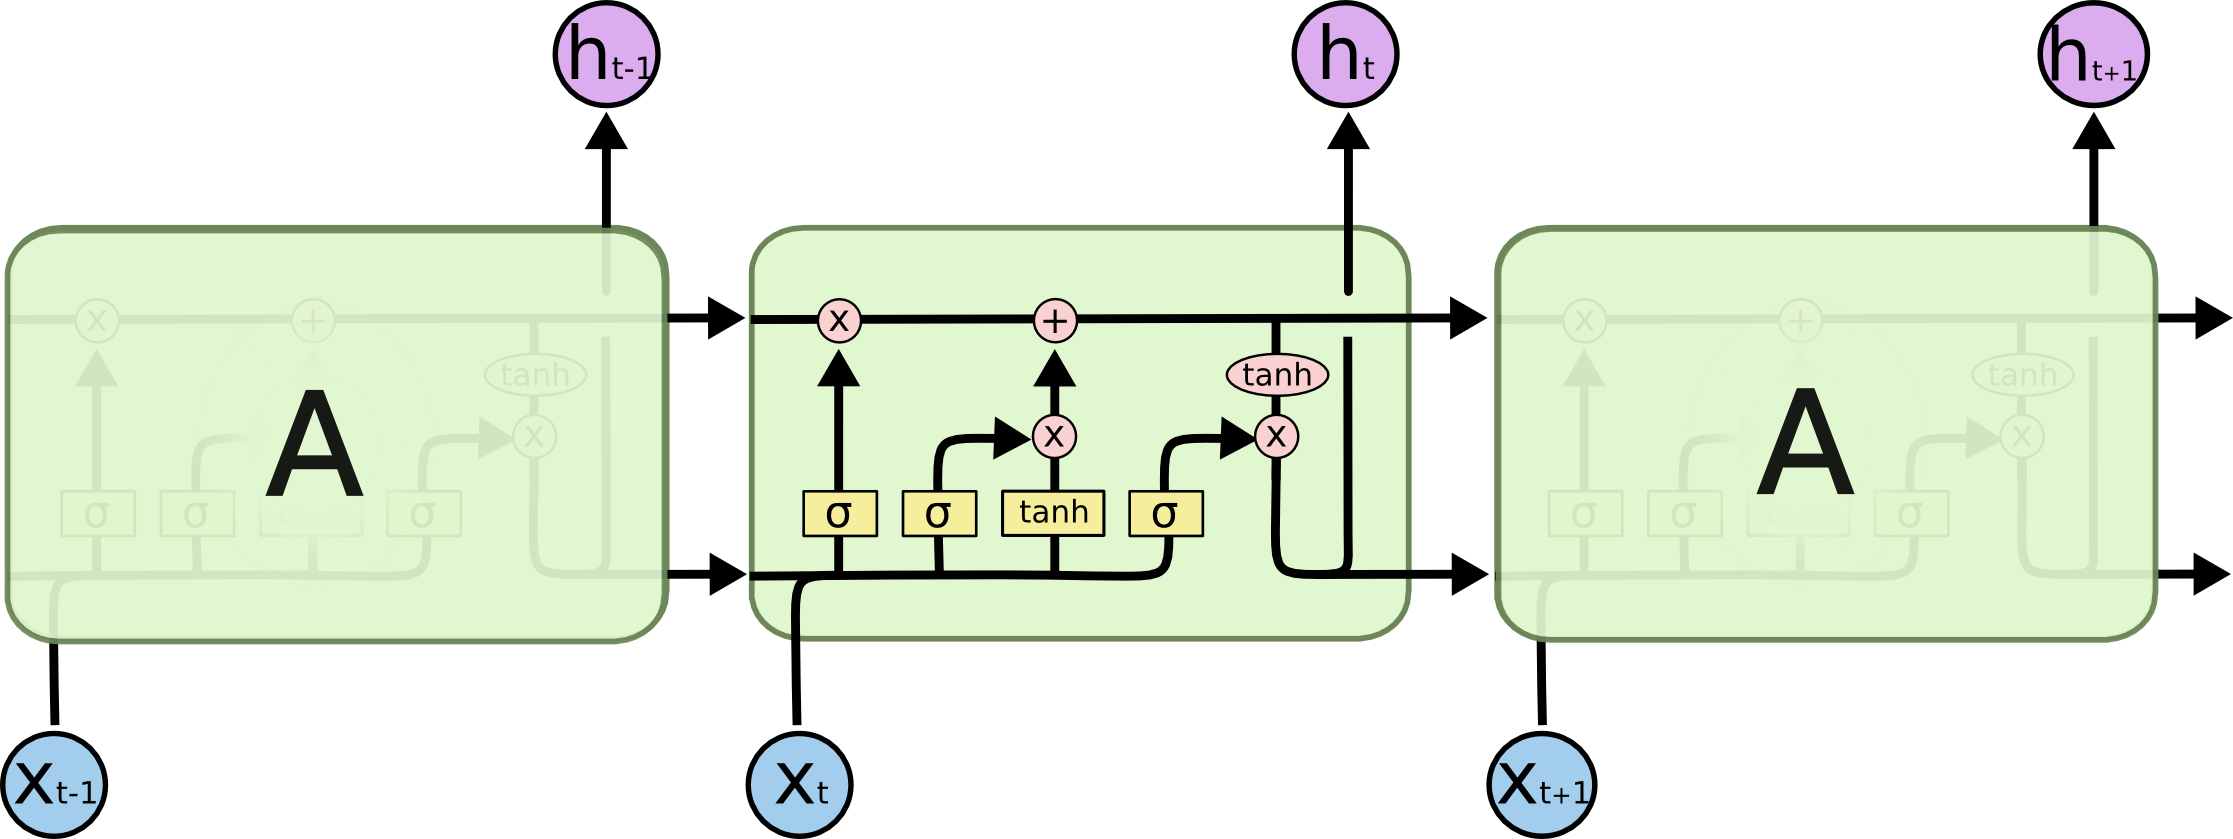
\includegraphics[width=0.8\linewidth]{img/stateofart/lstm_chain}
\end{center}
\caption{Example of the Architecture of a Convolutional Neural Network}
\label{fig:lstm_chain}
\end{figure}

Talk about paper that use LSTM

Another implementation of Recurrent Neural Network is a cell called Gated Recurrent Unit (GRU)\cite{cho2014learning}. This is a slightly more dramatic variation of the LSTM which combines the forget and input gate into an update gate and has been applied in the task of video classification\cite{ballas2015delving} in conjunction with CNNs.

\section{Convolutional Neural Networks for Activity Classification}

Talk about the 

%%%% Comments
Now talk about the recurrent neural network architecture proposed in the different papers of the state of the art. Talk about what RNN and LSTM are, some equations?

% AMAIA: Don't use equations in the state of the art. Maybe later in the methodology

Talk about some architectures interesting in the activity detection field and explain them more detailed (not much detailed but a little)??

% AMAIA: Yes, definitely ! I think that what you will explain in later sections is primarily focused on detection, so it is relevant that you explain what people have done in the past, and how your approach differs from them. I think what is interesting in your work is that you don't train in several stages using segment candidates. You train a single network. Ok, it does not improve the results, but the approach is much nicer ideally. 


